\documentclass[conference]{IEEEtran}
\usepackage{lipsum}
\IEEEoverridecommandlockouts
\usepackage{cite}
\usepackage{amsmath,amssymb,amsfonts}
\usepackage{algorithmic}
\usepackage{graphicx}
\usepackage{textcomp}
\usepackage{hyperref}
\usepackage{xcolor}
\usepackage{listings}
\lstset{basicstyle=\ttfamily,
  showstringspaces=false,
  commentstyle=\color{red},
  keywordstyle=\color{blue},
  literate={~} {\texttildelow}{1},
  tabsize=2,
  keepspaces=true,
  otherkeywords={curl, linkerd, kubectl, minikube}
}

\def\BibTeX{{\rm B\kern-.05em{\sc i\kern-.025em b}\kern-.08em
    T\kern-.1667em\lower.7ex\hbox{E}\kern-.125emX}}

\makeatletter
\newcommand{\linebreakand}{%
  \end{@IEEEauthorhalign}
  \hfill\mbox{}\par
  \mbox{}\hfill\begin{@IEEEauthorhalign}
}
\makeatother

\newcommand{\linkerd}{\textsc{Linkerd}}
\newcommand{\traefik}{\textsc{Traefik}}
\newcommand{\kubernetes}{\textsc{Kubernetes}}

\begin{document}

\title{Service Meshes as a Solution for Developing Technology-independent Microservices
}

\author{

\IEEEauthorblockN{Dangendorf, Kilian}
\IEEEauthorblockA{\textit{ Angewandte Informatik (M. Sc.)} \\
\textit{Hochschule Hannover}\\
kilian.dangendorf@stud.hs-hannover.de}
\and
\IEEEauthorblockN{Kirch, Eike}
\IEEEauthorblockA{\textit{ Angewandte Informatik (M. Sc.)} \\
\textit{Hochschule Hannover}\\
eike.kirch@stud.hs-hannover.de}
\and
\IEEEauthorblockN{Rust, Christopher}
\IEEEauthorblockA{\textit{ Angewandte Informatik (M. Sc.)} \\
\textit{Hochschule Hannover}\\
christopher.rust@stud.hs-hannover.de}
\linebreakand 
\IEEEauthorblockN{Ottlik, Manuel}
\IEEEauthorblockA{\textit{ Angewandte Informatik (M. Sc.)} \\
\textit{Hochschule Hannover}\\
manuel.ottlik@stud.hs-hannover.de}
}

\maketitle
\thispagestyle{plain}
\pagestyle{plain}

\begin{abstract}
\lipsum[100]
\end{abstract}

% brauchen wir sowas?
\begin{IEEEkeywords}
service meshes, microservices, kubernetes, python, istio, linkerd, nodejs, scalability, high availability
\end{IEEEkeywords}

\section{Introduction}

A microservice is an autonomous service that maps a small task of a specific domain and provides message-based communication through a well-defined interface \cite[p. 18]{microservices-general}.

High autonomy, cohesion, and interoperability are among the quality characteristics of a microservice. High autonomy of microservices ensures that the application is independent, self-contained, and fail-safe. High cohesion is hoped to increase maintainability and fast localization of errors. Interoperability ensures speeding up integrations \cite[p. 208 ff.]{microservices-general}.

Powerful microservices frameworks such as Spring Boot or Spring Cloud represent common solutions for microservices development. Key goals such as high availability, scalability, and resilience are achieved by providing services such as circuit breaking, load balancing, and API gateways \cite{spring-cloud}. These services are provided by using a framework, which is usually bound to a single programming language.

However, this contradicts the technology independence approach \cite{from-monolith} to microservices. This paper aims to shed light on whether and how service meshes can provide a solution to this problem.

\section{challenges of microservices}

The essential characteristic of a microservice architecture is to develop an application as a set of small and independent services. These run within their own process and are developed and deployed independently. Figure \ref{fig:microservice} illustrates the granularity of the microservice layer, where the business logic is designed to be very atomic. Each microservice should ideally have its focus on business logic \cite[p. 7]{sm3}.

Because of the granularity, the need for interservice communication increases. The complexity of this communication is usually more challenging than the actual business logic implementation. Due to the increased inter-service communication, microservices tend to be more prone to failures. This results in the requirement that a failure of one or more of these services should not bring down the entire application. Therefore, a failure of a microservice should be handled in such a way that it has minimal impact on the business functionalities of the application \cite[p. 11 ff.]{sm3}.

\begin{figure}
    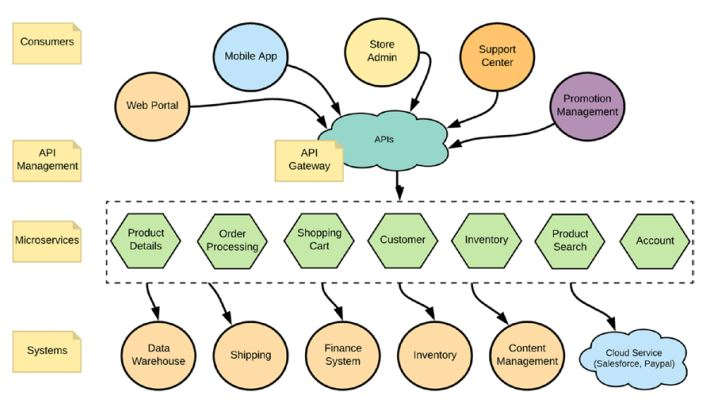
\includegraphics[width=\columnwidth]{img/microservice.JPG}
    \caption{Ex. microservice architecture of an online retail application \cite[p. 7]{sm3}}
    \label{fig:microservice}
\end{figure}

Another important challenge in the microservice context is maintenance. Due to the complexity of the architecture, it is necessary to introduce appropriate tools for e.g. service monitoring \cite[p. 16]{sm3}.
\section{Introduction to Docker and Kubernetes}

According to Google Trends, one of the most widespread solutions for microservices is \textsc{Kubernetes}.
To understand practical solutions of service meshes, it is very helpful to know how \textsc{Kubernetes} works. Since \textsc{Kubernetes} is often used together with \textsc{Docker}, this tool is also briefly explained.

\subsection{Docker}

\textsc{Docker} is a tool to encapsulate applications in so-called containers. It is built on Linux user groups and namespaces. Compared to a virtual machine, \textsc{Docker} is much more lightweight. All containers on the same host machine share the operating system kernel. Therefore, the overhead of booting the operating system for each container is eliminated \cite[p. 220 ff.]{sm3}.

Microservices are often deployed as so-called \textsc{Docker} images. This is a package consisting of the application and all its dependencies. The application itself only has access to the dependencies running in the image. The build process of a \textsc{Docker} image is defined in a so-called \textsc{Dockerfile} \cite[p. 224]{sm3}.

\subsection{Kubernetes}

\textsc{Kubernetes} provides a number of functions. It can be seen as a container platform, microservices platform and cloud platform.
It is a common way to use container technologies nowadays. Containers are isolated; they do not have access to processes or file systems of the host or other containers.
Advantages of container solutions are easy creation and deployment of container images that allow continuous integration, delivery and test. The role of \textsc{Kubernetes} is to manage and orchestrate these containers \cite{k8s}.

The four main \textsc{Kubernetes} objects are important to understand the role of service meshes in the microservices context:
\begin{itemize}
\item Pods: Pods are the smallest deployable unit that \textsc{Kubernetes} manages. A pod is one or a group of multiple containers that share storage and network resources.
\item Namespaces: Pods can be grouped into what are called namespaces. These represent a kind of virtual cluster. This already represents a kind of security concept. By default, a service from namespace A cannot communicate with a service from namespace B without explicit configuration.
\item Labels: Each \textsc{Kubernetes} deployment can be attached with an arbitrary amount of labels. These labels are simple key/value pairs that allow to group objects in \textsc{Kubernetes} into subsets \cite{k8s}.
\end{itemize}
\section{Characteristics of Service Meshes}

\begin{figure*}
    \centering
    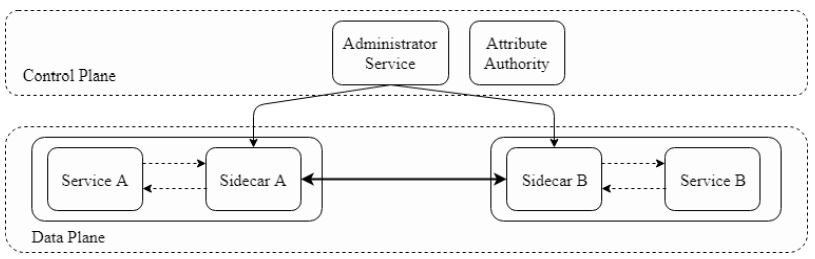
\includegraphics[width=0.8\textwidth]{img/mesh_detailed.JPG}
    \caption{Control and data plane in a service mesh\cite{sm4}}
    \label{fig:detailed mesh}
\end{figure*}


\begin{figure}
    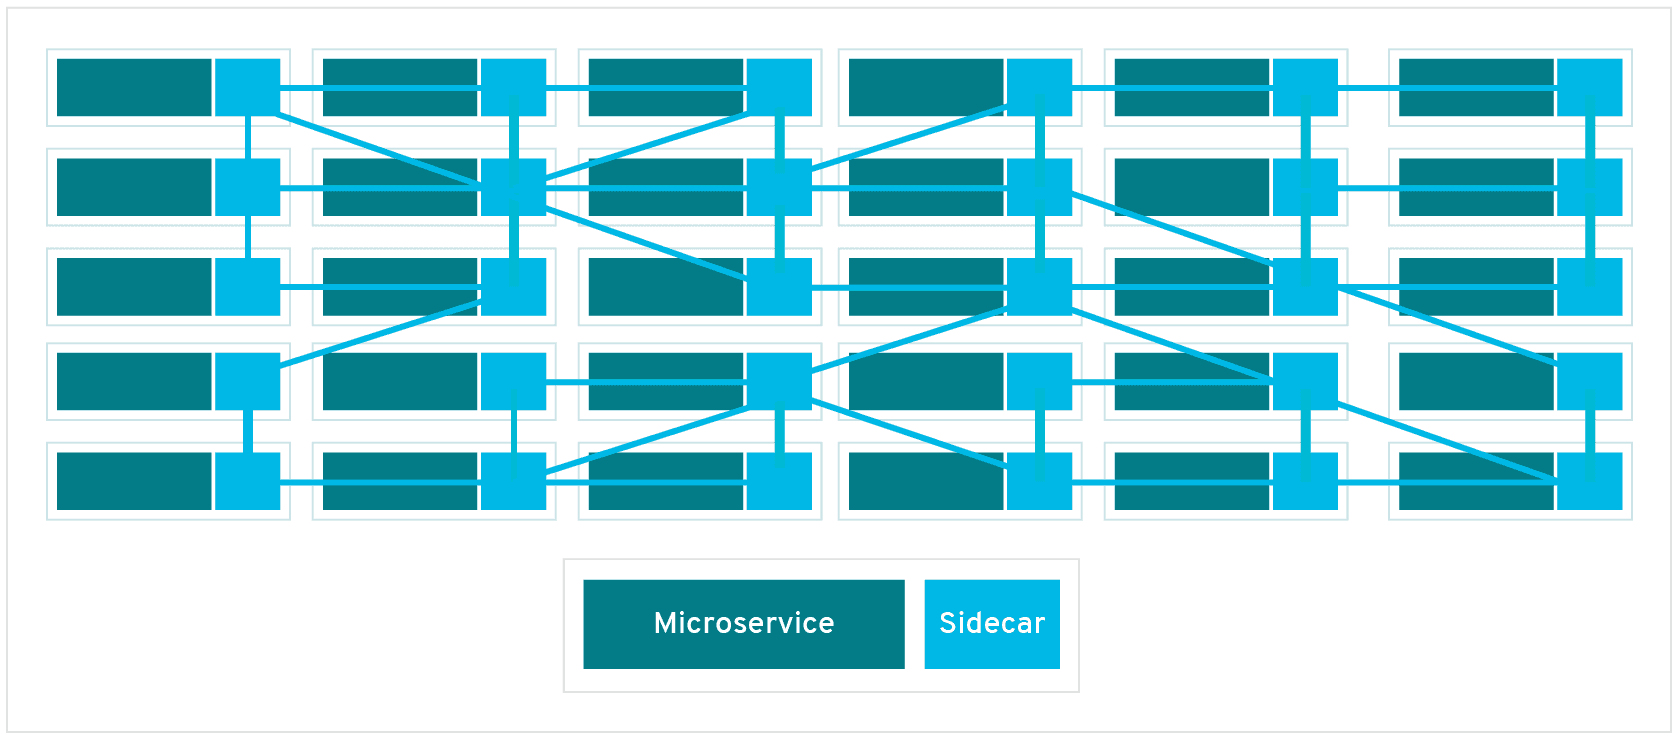
\includegraphics[width=\columnwidth]{img/mesh.png}
    \caption{Simplified service mesh based microservice architecture \cite{sm2}}
    \label{fig:overview}
\end{figure}

Chapter \ref{chap:microservices} may have already given the impression that developing infrastructure services for microservices can be more complex than implementing the business logic itself. For this reason, there is a need for solutions in which infrastructure and business logic are separated in order to reduce the burden on the developer. A service mesh is one conceivable solution approach that also provides an interface which makes infrastructure tasks more comprehensible. It is defined as follows:

\subsection{Definition}

According to \cite{sm1}, a service mesh is a dedicated infrastructure layer which handles inter-service communication. This infrastructure layer is basically a composition of several lightweight network proxies, so-called sidecars. This pattern is explained in the next chapter.  Furthermore, a service mesh is responsible for reliably delivering requests in a complex microservice topology.

The idea of service meshes sounds very promising: The developer no longer has to worry about the infrastructure tasks. In the context of this paper it should become clear how decoupled the infrastructure layer actually is.

\subsection{Sidecar Pattern}

According to the service mesh definition, lots of service mesh solutions take usage of the so-called Sidecar pattern to realize the network proxies.

According to a Sidecar pattern definition from \cite{sm3}, a sidecar is a software component that is located alongside the actual software, but runs within a dedicated process. All logic that is not part of the business logic is handled by the sidecar. Typically, the sidecar also handles incoming and outgoing communication. This is a good approach for clean separation of concerns.

\subsection{Architecture}
\label{chap:mesh-architecture}

Figure \ref{fig:overview} shows a simplified microservice architecture using service meshes. The mentioned infrastructure layer is a composition of the lightweight network proxies. These sidecars control the entire network communication between the microservice instances. Without service mesh, each service must implement this interservice logic on its own, which compromises developer focus on business goals. The figure perfectly illustrates that application services are decoupled from interservice communication.

A more detailed illustration of a service mesh architecture is shown in figure \ref{fig:detailed mesh}. A service mesh consists of a control plane and a data plane.
The control plane is responsible for administrative tasks. This is where, for example, system-wide authentication and authorization policies are configured and made available to the proxies. Furthermore, settings for circuit breaking, timeouts and load balancing are made here. The composition of all application services with their sidecar proxies is called data plane \cite{sm4}.

\subsection{Worth of Technology Independence}

Listing \ref{lst:java-cb} shows a short and simplified example for a dummy application that is wrapped by a circuit breaker. The problems with this approach are obvious: If one decides to disable mechanisms such as circuit breaking etc., this basically means that the implementation of the application has to be adapted, tested and re-deployed. This effort is not insignificant in large applications. 

\begin{lstlisting}[basicstyle=\footnotesize ,language=java,caption={Circuit breaker example with Spring Cloud + Hystrix \cite{hystrix-ex}}, label={lst:java-cb}]
@Service
public class BookService {

  private final RestTemplate restTemplate;

  public BookService(RestTemplate rest) {
    this.restTemplate = rest;
  }

  @HystrixCommand(fallbackMethod = "reliable")
  public String readingList() {
    URI uri = URI
        .create("http://localhost:8090/recommended");

    return this.restTemplate
        .getForObject(uri, String.class);
  }

  public String reliable() {
    return "Cloud Native Java (O'Reilly)";
  }

}
\end{lstlisting}

Microservices that use services meshes are technology-independent and can therefore do without libaries from, for example, the Netflix OSS stack. Keeping the option of technology independence open can even make sense if the entire application is written in a single language such as Java, for example. If you are thinking about deploying a new version or library, you could limit this to just a few services. The risk of breaking existing functionalities is thus limited, which makes it much easier to keep one's own stack modern. Netflix, for example, has discontinued support for Hystrix \cite{hystrix-eol}. Microservice operators that do not run a service mesh would now have to look for another framework and adapt the implementation of their services.

\subsection{Central Tasks}

Each service mesh has specific tasks to solve to enable microservice operation. These are named and briefly introduced below \cite{sm1}:

\subsubsection{Service Discovery}

The number of service instances and the states and configurations change more frequently. For this reason, middleware is required to serve as an intermediary. It would be very complicated if every service A had to know under which IP and which port it can reach service B.

\subsubsection{Load Balancing}

A load balancer is necessary to skillfully distribute requests to a service among replicas when loads are higher.

\subsubsection{Fault Tolerance}

The microservice application must not be overly dependent on individual replicas being in a faulty state. For this reason, the service mesh must solve the task of forwarding requests only to services that have a sufficient health state.

\subsubsection{Traffic Monitoring}

All communication between all microservices must be recorded and made visible, for example, via a central dashboard. In addition to logging, it makes sense to display metrics and statistics for the individual services.

\subsubsection{Circuit Breaking}
One of the difference between in-memory calls and remote calls is, that remote calls might fail due to connection problems or long-running operations that lead to a timeout. The solution for this problem is not to just avoid bugs, errors and connection problems: Microservices need to be resilient. One way to do this is to implement the circuit breaker pattern. If recurring connection errors are detected for a resource, access to this resource is blocked by the circuit breaker so that it is not overloaded further.

\subsubsection{Authentication and Access Control}

With the use of a service mesh, it should be easy to apply and remove certain policies for authentication and authorization. One such policy could be that access to Service A, which provides the database logic, is only allowed by Service B and no one else.

\subsection{Opportunities and Risks}

\begin{figure}
    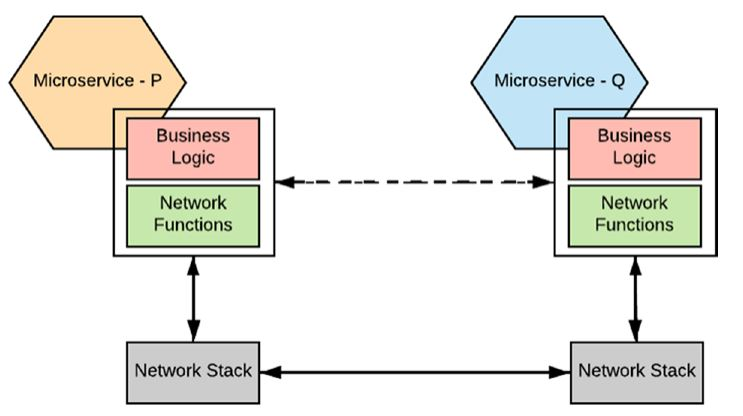
\includegraphics[width=\columnwidth]{img/microservices_without_mesh.JPG}
    \caption{Ex. architecture of microservices without service mesh\cite[S. 265]{sm4}}
    \label{fig:microservice-without-mesh}
\end{figure}

To highlight the benefits of a services mesh, you need to imagine a microservice architecture without services meshes. Figure 4 illustrates that each microservice requires a significant amount of logic to enable interservice communication. The effort required to implement this logic multiplies if, for example, Circuit Breaker is required in Java, Node.js, and Python. Since the requirements for infrastructure logic are the same in almost all microservice applications, it only makes sense to map this logic to an abstracted layer. This is where the service mesh comes into play. According to \cite{sm4}, the further advantages and drawbacks of a service mesh are as follows:

\subsubsection{Advantages}

\begin{itemize}

    \item Developers can concentrate on implementing their business applications. The management of a service mesh is more the task of an administrator or DevOps engineer.

    \item Polyglot support is another key benefit of service meshes. Developers can use their favorite programming languages and frameworks while still benefiting from the features provided.

    \item In addition, the monitoring of services works out of the box. Distributed tracing and metrics require no additional effort from the developer's perspective. Furthermore, the application is decentralized, but centrally maintainable through the control plane. 

\end{itemize}
\subsubsection{Drawbacks}

\begin{itemize}
    \item On the other hand, service meshes also have disadvantages. Of course, the complexity of the architecture increases significantly by adding a sidecar proxy to each service instance. This also leads to the fact that each service call requires an additional hop.
    \item In addition, there are some problems in inter-service communication that service meshes do not address. These include complex routing, type mapping, and integration of other services and systems.
    \item A final important point is that service meshes are a comparatively new technology. The solutions are not necessarily mature enough for highly scaling environments.
\end{itemize}








\section{Solutions on the market}

The following chapter presents the two most popular solutions used in the context of service meshes: \textsc{Istio} and \textsc{Linkerd}. Both technology solutions have in common that they are based on \textsc{Kubernetes}. While \textsc{Linkerd} requires \textsc{Kubernetes}, \textsc{Istio} could also rely on virtual machines.

Service meshes that use \textsc{Kubernetes} extend the functionality by abstracting concepts like automatic sidecar injection. This would be also possible without service meshes, but significantly more complex and less automated.

\subsection{Istio}

As illustrated in figure \ref{fig:arch-istio}, \textsc{Istio} uses a basic control and data plane architecture, as explained in chapter \ref{chap:mesh-architecture}. For the data plane, it uses the sidecar pattern by using \textsc{Envoy} proxies. \textsc{Envoy} a high-performance proxy that already brings features like service discovery, load balancing, circuit breaking and many more \cite{istio-docs-arch}.

\textsc{Istiod} (Istio daemon) provides management for service discovery, configuration and certificates. It converts routing rules into \textsc{Envoy}'s configuration format and also directs the traffic to the sidecar proxies \cite{istio-docs-arch}.

\begin{figure}
    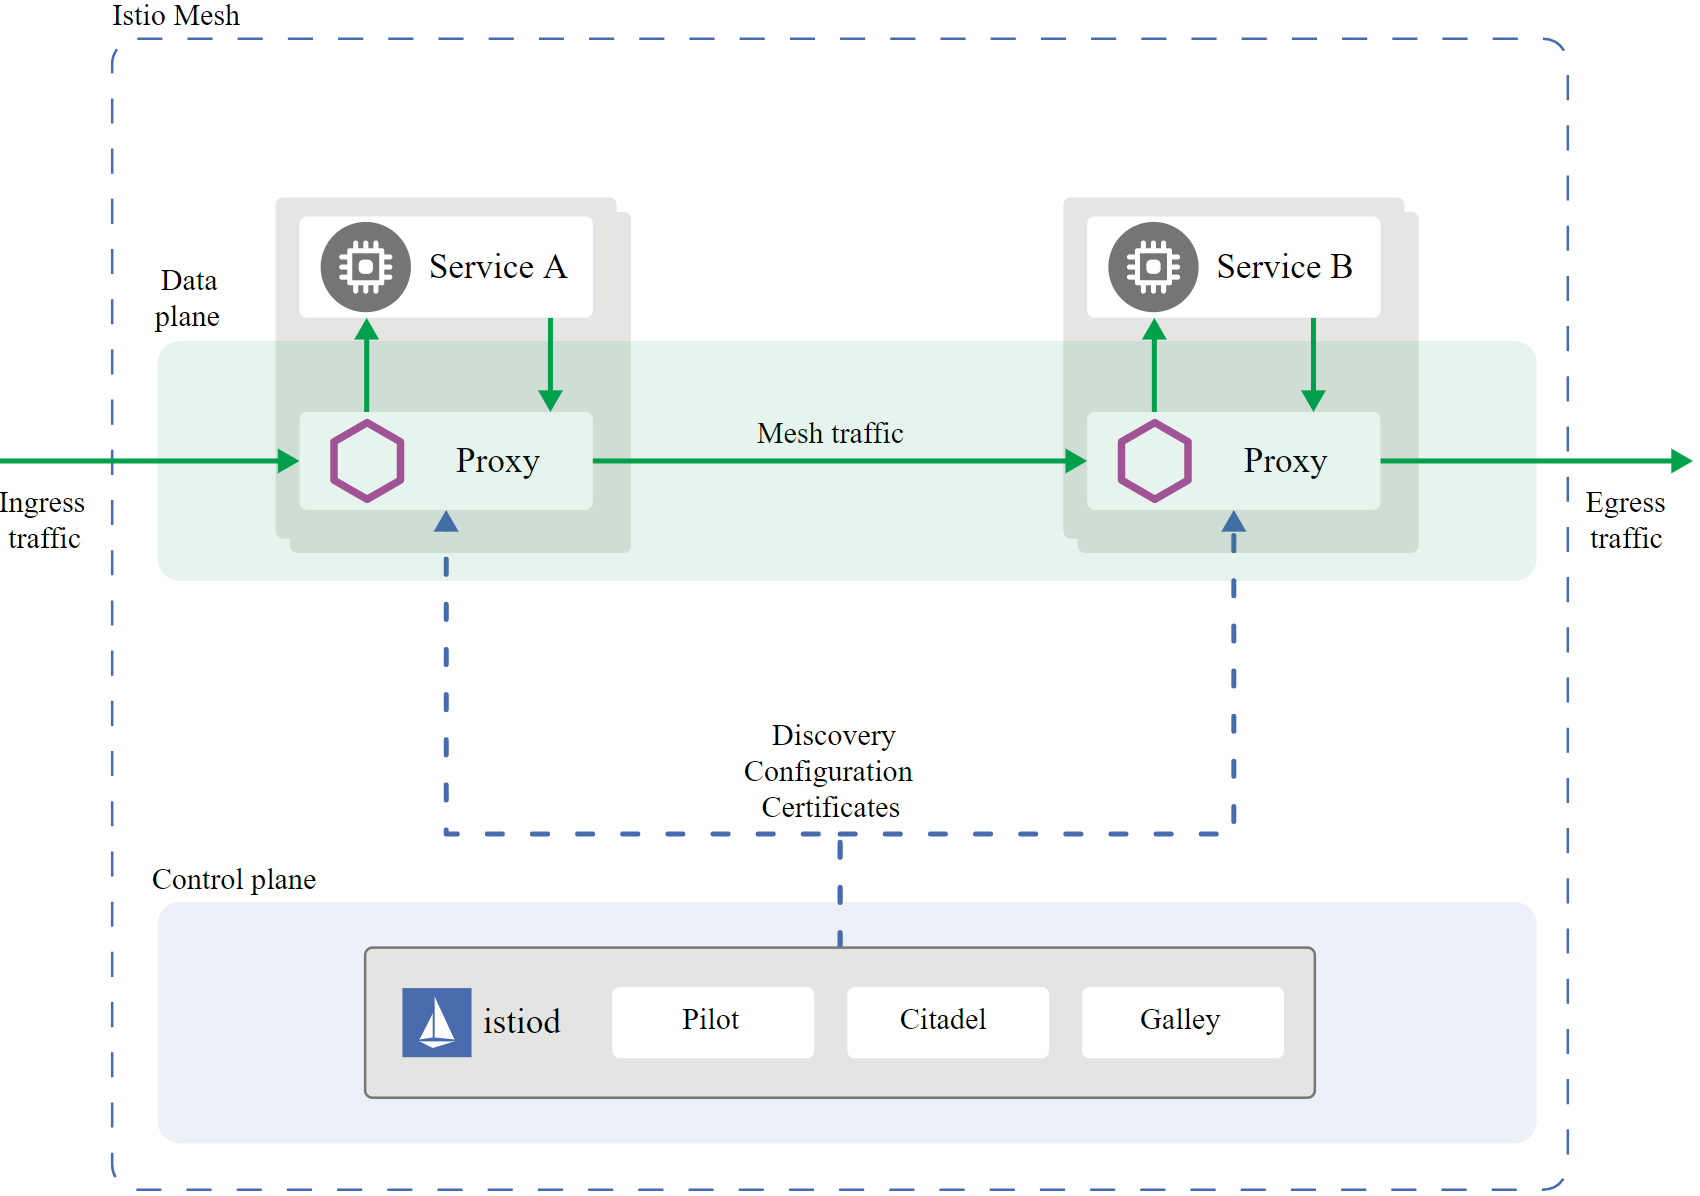
\includegraphics[width=\columnwidth]{img/istio_architecture.png}
    \caption{Architecture of \textsc{Istio} \cite{istio-docs-arch}}
    \label{fig:arch-istio}
\end{figure}

\subsection{Linkerd}
\label{linkerd}
According to \textsc{Linkerd}'s documentation \cite{linkerd-docs-arch}, \textsc{Linkerd} also uses a basic control and data plane architecture, as explained in chapter \ref{chap:mesh-architecture}. It also uses the sidecar pattern, but has implemented an own proxy solution named \textsc{Linkerd2-proxy}. \textsc{Linkerd} developers rate \textsc{Envoy} as too complex \cite{linkerd-docs-no-envoy}, which is why they decided to implement their own solution, which they call a "micro-proxy". 
Unlike \textsc{Istio}, \textsc{Linkerd} does not handle ingress traffic. It works in conjunction of every ingress controller of choice, e.g. \textsc{nginx} or \textsc{traefik} \cite{linkerd-docs-faq}.

As illustrated in figure \ref{fig:arch-linkerd}, each \textsc{linkerd-proxy} has access to two components: \textsc{identity} and \textsc{destination}.

\textsc{destination} is a lookup-service, where each proxy is able to check where exactly to send requests. \textsc{identity} provides a certificate authority.

While injecting a sidecar proxy on an application service, a route \textsc{/metrics} at port 4191 is exposed to provide log messages and metrics for \textsc{Prometheus}, which is a central logging and monitoring instance which is often used with \textsc{Kubernetes} \cite{linkerd-docs-arch}.

\begin{figure}
    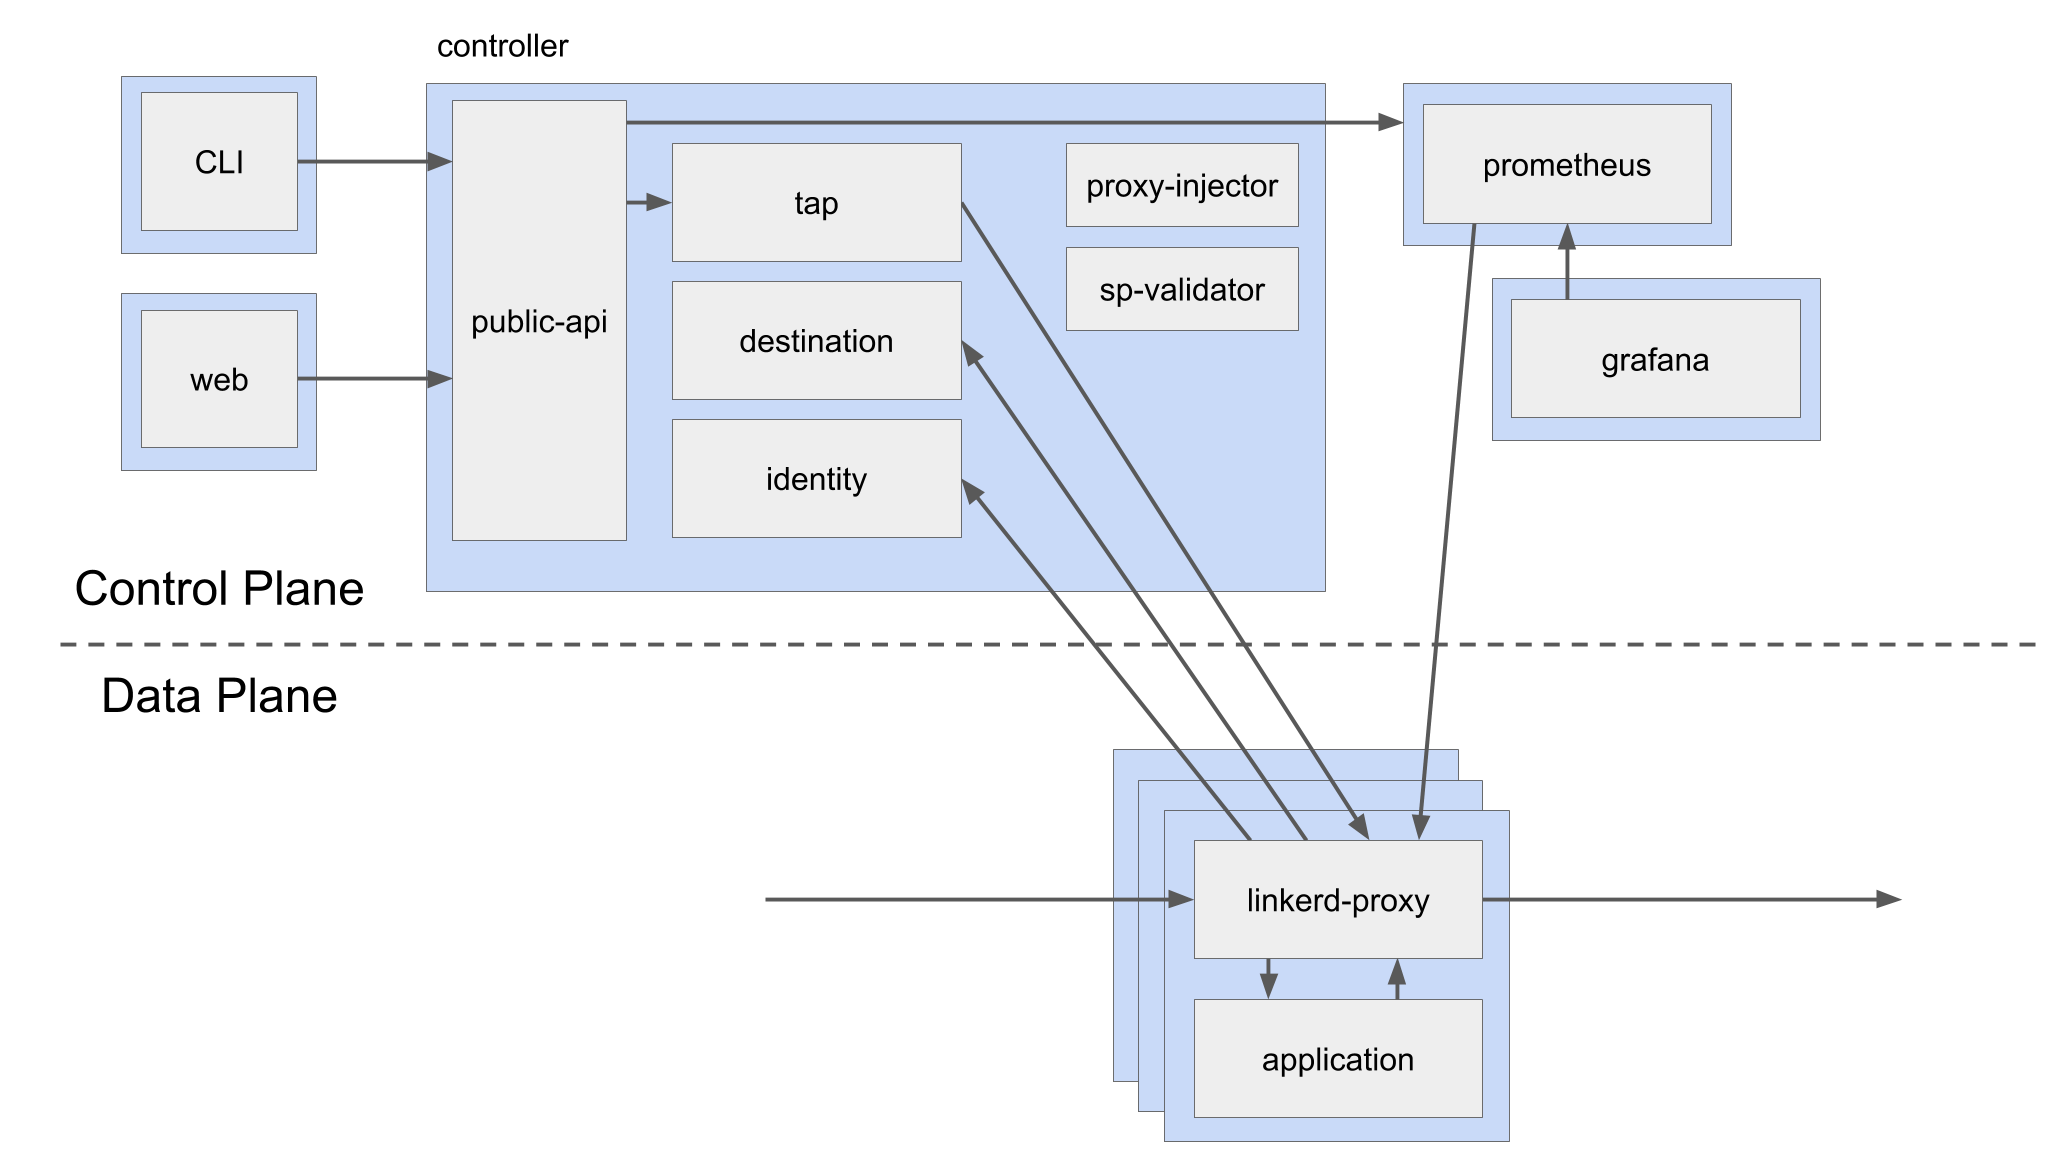
\includegraphics[width=\columnwidth]{img/linkerd_architecture.png}
    \caption{Architecture of \textsc{Linkerd} \cite{linkerd-docs-arch}}
    \label{fig:arch-linkerd}
\end{figure}

\subsection{Comparison}

As stated before, two very popular solutions for service meshes are \textsc{Linkerd} and \textsc{Istio}. Table \ref{tab:istio-linkerd} summarizes the key aspects of both tools, according to \cite{linkerd-github}, \cite{istio-github}, \cite{istio-linkerd-compare-1} and \cite{istio-linkerd-compare-2}:

\begin{table}
\centering

\begin{tabular*}{\columnwidth}{c|c|c}
                                 & Istio                                                                                                              & Linkerd     \\\hline
Initiators & \begin{tabular}[c]{@{}c@{}}Lyft, IBM,\\Google\end{tabular}                                                          	& \begin{tabular}[c]{@{}c@{}}Buoyant, Cloud Native\\Foundation\end{tabular}                                                           \\\hline
License                 & \multicolumn{2}{c}{Apache 2.0}                                                                                                          \\\hline
Runs on                          & \begin{tabular}[c]{@{}c@{}}Kubernetes,\\VMs\end{tabular}                                                           & Kubernetes  \\\hline
Sidecar proxy                    & \multicolumn{2}{c}{Yes}                                                                                                          \\\hline
Supports mTLS                    & \multicolumn{2}{c}{Yes}                                                                                                          \\\hline
Certificate management           & \multicolumn{2}{c}{Yes}                                                                                                          \\\hline
Authentication and authorization & \multicolumn{2}{c}{Yes}                                                                                                          \\\hline
Blue/Green deployment            & \multicolumn{2}{c}{Yes}                                                                                                          \\\hline
Circuit breaking                 & Yes                                                                                                                & No          \\\hline
Fault injection                  & \multicolumn{2}{c}{Yes}                                                                                                          \\\hline
Rate limiting                    & \multicolumn{2}{c}{Yes}                                                                                                          \\\hline
Monitoring                       & \multicolumn{2}{c}{Yes, with Prometheus}                                                                                         \\\hline
Complexity                       & High                                                                                                               & Low         \\\hline
Starts on GitHub \cite{linkerd-github} \cite{istio-github}              & 26.2k & 6.6k        \\\hline
Open issues on GitHub \cite{linkerd-github} \cite{istio-github}                 & 817                                                                                                                & 257         \\\hline
Documentation                    & ++                                                                                                                 & +          
\end{tabular*}
\vspace{0.25mm}
\caption{Comparison between Isto and \textsc{Linkerd}}
\label{tab:istio-linkerd}
\end{table}


%
%
% Mehr Erklärung zu Linkerd?
%
%

From an operators perspective, \textsc{Istio} and \textsc{Linkerd} look quite similar. After installing the service mesh, there are two main usage aspects: One the one hand, operators need to inject sidecar proxies in the pods of the microservice. On the other hand, they need to apply pluggable resources in YAML format, that could define policies like the usage of TLS.

By executing the command listed in \ref{lst:istio}, all deployments from namespaceA automatically get a sidecar proxy injected, while listing \ref{lst:linkerd} shows the injection command of a single deployment when using \textsc{Linkerd}.

\begin{lstlisting}[language=bash,caption={Injection of sidecards into deployments of a namespace in \textsc{Istio}},label={lst:istio}]
#!/bin/bash
kubectl label namespace default \
	istio-injection=enabled
\end{lstlisting}

\begin{lstlisting}[language=bash,caption={Injection of sidecards into a deployment in \textsc{Linkerd}}, label={lst:linkerd}]
#!/bin/bash
cat deployment.yml | linkerd inject - \
	| kubectl apply -f -
\end{lstlisting}

%
% TODO: WRITE STUFF
% 

As table \ref{tab:istio-linkerd} clarifies, \textsc{Linkerd} seems to be less complex and more lightweight compared to \textsc{Istio}. One missing key feature of \textsc{Linkerd} is circuit breaking, which is requested by users and currently under development \cite{linkerd-circuit-breaker}. Nevertheless, \textsc{Istio} seems to be more powerful and mature, has more users and functionalities. Along with this, the pool of tutorials and documentation is also larger.
We will choose \textsc{Linkerd} because of its lightweight nature. The setup of \textsc{Linkerd}'s hello world example looks pretty straight forward and suitable and appropriate for a proof of concept. Since \textsc{Linkerd} suggests to use \textsc{traefik} as an ingress controller \cite{linkerd-traefik}, we will use it as well.
\section{Prototypical service mesh implementation}

The following chapter describes our concept of our prototypical service mesh implementation and its outcome. In order to also practically work out the differences between service meshes and a traditional microservice operation, we will initially run our application using only Kubernetes, and then later set up a service mesh.

\begin{figure*}
    \centering
    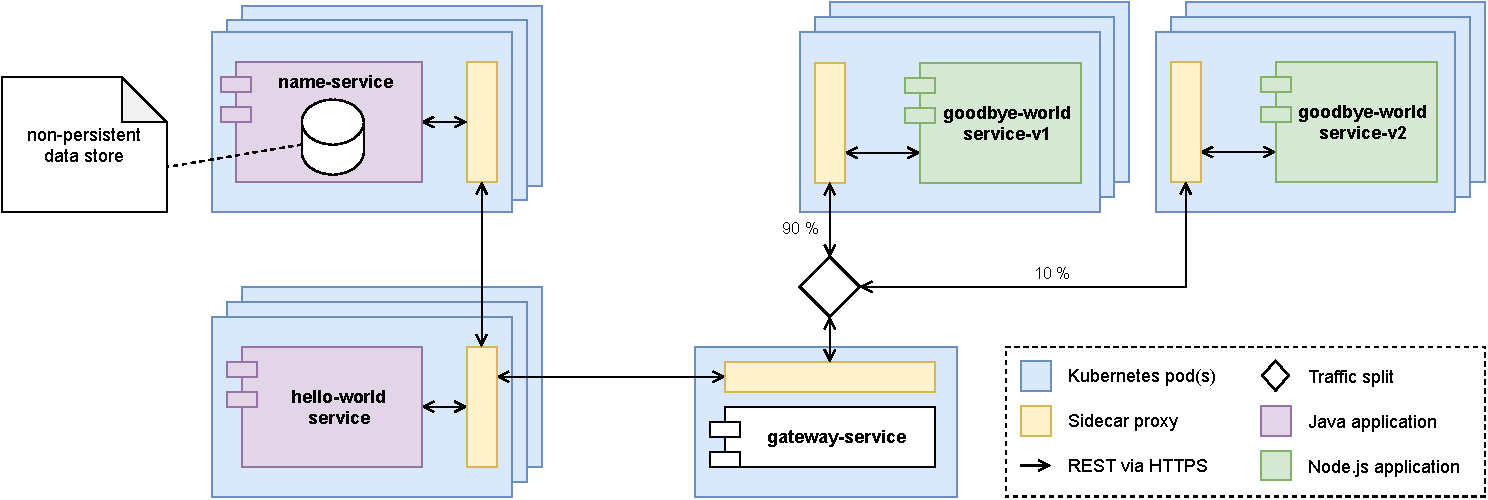
\includegraphics[width=\textwidth]{img/diagram-draft.pdf}
    \caption{Architecture overview of the PoC application}
    \label{fig:poc-overview}
\end{figure*}

\subsection{Services}

Our basic idea is to implement three simple microservice applications that communicate via REST. To prove technology independence, one service is written in Node.js, while the other two services are written in Python. Another requirement to meet is that the services have to be as simple as possible. Furthermore, the functionality of the services is intended to be as follows:

\begin{itemize}
\item \textsc{name-service}: Provides endpoint to retrieve a collection of names. It stores the names in a file or a simple array list.
\item \textsc{goodbye-world-service}: Provides endpoint to retrieve a message ``Goodbye, World!"
\item \textsc{hello-world-service}: Contacts the \textsc{name-service} and provides an endpoint that returns a ``Hello, \{name\}" message for each name object from name service.
\end{itemize}

Since Linkerd does not provide an own ingress controller (see chapter \ref{linkerd}), we use an external ingress controller named \textsc{traefik}.

\subsection{Showcases}

Our prototypical implementation aims to provide answers to the following five challenges of running and maintaining microservices.

\subsubsection{Encryption}

By using a service mesh, it should be shown that an encryption policy can be easily applied or removed.

\subsubsection{Canary Deployment}

To provide an example showcase for canary deployment, we implemented two versions of \textsc{goodbye-world-service} which differ minimally by the returned string. The mesh is tasked with redirecting traffic so that 90\% of all requests are made to version 1 and 10\% of requests are made to version 2.

\subsubsection{Access Policies}

Another restriction is that the \textsc{name-service} is only accessible from the \textsc{hello-world-service}. Access restriction should not be a task of the actual \textsc{name-service} application. We want to show that access to services is easily managable via YAML resources.

\subsubsection{Central monitoring and logging}
The proof of concept should show that services in a microservice landscape can be monitored and managed centrally using the service mesh.

\subsection{Setup of Linkerd}

The following sequence of bash commands shows the \textsc{Linkerd} installation process and the application of the service mesh to the \textsc{Kubernetes} cluster \cite{linkerd-get-started}:
\begin{lstlisting}[language=bash,caption={Setup of \textsc{Linkerd}}, label={lst:linkerd-setup}]
#!/bin/bash
curl -sL https://run.linkerd.io/install \
	| sh
export PATH=$PATH:$HOME/.linkerd2/bin
echo "export PATH=$PATH:$HOME/.linkerd2/bin" \
	>> ~/.bashrc
linkerd install | kubectl apply -f -
\end{lstlisting}

\begin{itemize}
	\item Install linkerd
\begin{itemize}
	\item wir kümmern uns nicht um Verschlüsselung; das macht Linkerd
	\item linkerd install | Kubectl apply -f -
	\item ab diesem Moment mTSL aktiviert
	\item Pipes
\begin{itemize}
	\item this is a usual workflow: Linkerd’s output is a yaml-file, that can be piped into Kubectl 
\end{itemize}
\end{itemize}
	\item wie bekommen wir die µS's ins SM, 
\begin{itemize}
	\item similar to the installation we inject the Linkerd command:
	\item injecten $\rightarrow$ schon im Text drin
\begin{itemize}
	\item entweder einzeln, 
	\item oder für alle folgenden
\end{itemize}
	\item Linkerd parses the yaml file(s) and provides annotations.
\begin{itemize}
	\item Zeige Annotation in Listing
\begin{itemize}
	\item \lstinline|linkerd.io/inject: enabled|
\end{itemize}
\end{itemize}
	\item resulting annotated yaml-file is given to Kubectl as parameter in file option (-f)
\begin{itemize}
	\item dies erzeugt Linkerd-Proxy
\end{itemize}
\end{itemize}
	\item Kommunikation der µS
\begin{itemize}
	\item da im gleichen Namespace, kein Problem
	\item K8s sorgt dafür, dass sie im selben Netz sind
	\item erreichen durch K8s-DNS Namen
\begin{itemize}
	\item setzen sich immer so zusammen
\end{itemize}
	\item diese in yml setzen
	\item Listing?
	\item µS A kann nun die REST-API von µS B unter dieser DNS nutzen
\end{itemize}
	\item Monitoring kommt "out-of-box"
\begin{itemize}
	\item Linkerd kommt mit Prometheus und Grafana
	\item Wir können sehen, wer mit wem wieviel redet
	\item Bsp. Baum aus Linkerd? helloworld spricht mir nameapi?
\end{itemize}
	\item jetzt haben wir schon SM, mTLS und Monitoring 
	\item Ingress Controller
\begin{itemize}
	\item wie kommen wir nun von außen an unserer Services?
	\item wir brauchen einen Ingress Controller
	\item as stated in V-B we chose Traefik
	\item Der kann zwar mehr, aber mehr brauchen wir nicht 
	\item nutzen ihn nur als remote proxy "vor" unseren Services
	\item Wenn injected, nutzen wir Traefik auch als LoadBalancer
\begin{itemize}
	\item \url{https://linkerd.io/2/tasks/using-ingress/} $\rightarrow$ HONOR ;)
\end{itemize}
\end{itemize}
	\item für Detail bzgl Installation und Nutzung bzw. siehe Repo (Anhang)
\end{itemize}



\subsection{Resource definition for applications}

\subsection{Policy application}
\section{Implementation and Results}

This section examines necessary steps to apply the showcases stated in \autoref{sec:showcases-1} with \linkerd{}, how the results look like and some pitfalls we have overcome.

Since functionality and APIs vary in time, the following table shows the versions of technologies we use:
\begin{table}[h]
\centering	
\begin{tabular}{c|c}
	Technology & Version \\\hline
	\textsc{Docker} & 20.10.3\\\hline
	\textsc{Minikube} & 1.17.1\\\hline
	\kubernetes & 1.20.2\\\hline
	\linkerd & 2.9.3 \\
\end{tabular}
\vspace{0.25mm}
%\caption{Comparison between Isto and \textsc{Linkerd}}
\label{tab:versions}
\end{table}

Services are built into \textsc{Docker}-images.
To use only one machine for development we used \textsc{Minikube}.
Within this \kubernetes{} and \linkerd{} run.

\subsection{Showcases Implementation}
With the exception of "Acess Policies" we implemented and controlled with \linkerd{} the challenges stated in \autoref{sec:showcases-1}.

\subsubsection{Encryption}
From the second that a service is injected by \linkerd{} and applied to the cluster, all communication to that service is automatically encrypted.
This holds not only for our self-implemented communication but also for metrics- and tap-services.
Since the communication is proxied by \linkerd{} it activates certificate distribution and encryption out-of-box.

If you don't want to use this feature, you can disable by overwriting the \linkerd{} configuration.
The following command will generate an updated YAML-configuration you can apply in \kubernetes{}.
\begin{lstlisting}
linkerd upgrade \
  --disable-identity \
  --disable-tap
\end{lstlisting}
Note: Once this configuration is applied, there will be no encryption neither in communication between services nor in tap- and metrics-services.

\subsubsection{Canary Deployment}
\label{sec:canary-result}
In first place we have to deploy a new version of the \textsc{name-service} next to the existing one.
The deployment is done the same way but with a different name (\lstinline|nameapi-v2|).
New Version of \textsc{name-service} is similar to the old one but returns a different string (forename \textit{and} surname) while API stays the same.
There are no changes in \textsc{hello-world-service} necessary.

Until now the new version is not used.
We have to define a traffic split showed in \autoref{lst:traffic-split}.

\begin{lstlisting}[caption={YAML configuration of 90/10 traffic split. 90\% of requests are routed to \lstinline|nameapi| and 10\% to \lstinline|nameapi-v2|.}, label={lst:traffic-split}]
apiVersion: split.smi-spec.io/v1alpha1
kind: TrafficSplit
metadata:
	name: nameapi-split
spec:
	service: nameapi
	backends:
	- service: nameapi
		weight: 90
	- service: nameapi-v2
		weight: 10
\end{lstlisting}

In the \lstinline|spec|-section we define two backends for the service \lstinline|nameapi|.
The argument \lstinline|weight| defines a split ratio.
90\% of traffic should be routed to the existing service with the name \lstinline|nameapi|, 10\% to the new one \lstinline|nameapi-v2|.

Right after applying this configuration, \linkerd{} dashboard shows a new section for traffic splits.
In \autoref{fig:results-traffic-split-weights} \linkerd{} visualizes the routed requests.
We can see the defined weights and the current requests per second (RPS), that are split according.

\begin{figure}
	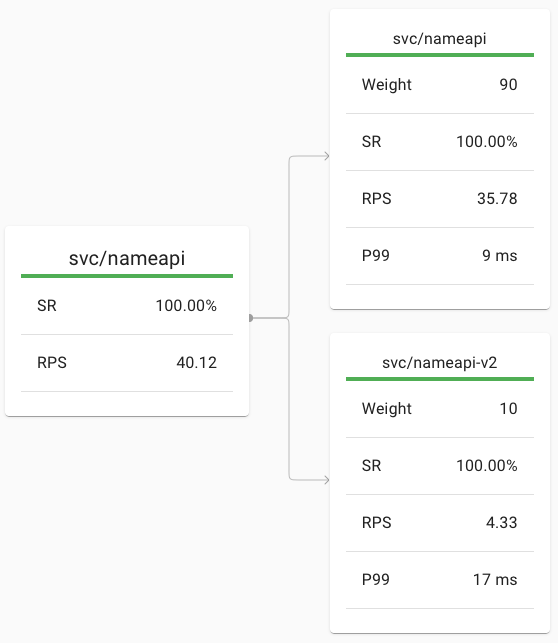
\includegraphics[width=\columnwidth]{img/results-traffic-split-weights}
	\caption{\linkerd{} dashboard displays the weights of the 90/10 traffic split.}
	\label{fig:results-traffic-split-weights}
\end{figure}

The \textsc{hello-world-service} stays unchanged, but requests the new version of \textsc{name-service} every tenth request without knowing.
The deployment section of \textsc{hello-world-service} in \linkerd{} dashboard now renders a delegation tree pictured in \autoref{fig:results-traffic-split-tree} showing that \textsc{hello-world-service} requests both versions of \textsc{name-service}.

\begin{figure}
	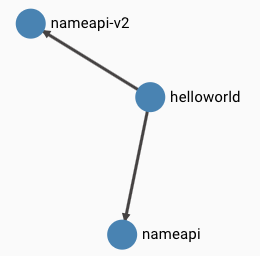
\includegraphics[width=.4\columnwidth]{img/results-traffic-split-tree}
	\centering
	\caption{Delegation tree of \textsc{hello-world-service} after traffic split.}
	\label{fig:results-traffic-split-tree}
\end{figure}




\subsubsection{Access Policies}
TBD

\subsubsection{Load Balancing}
\label{sec:load-result}
To show the integrated load balancing of \linkerd{} we defined three replicas of the \textsc{goodbye-world-service}.
Therefore we set In the deployment configuration at the \lstinline|spec|-section the count of replicas up to three	 (\lstinline|replicas: 3|).
Now \kubernetes{} will provide three pods running the \textsc{goodbye-world-service}.
Since we injected the configuration file by \linkerd{} all replicas are within the service mesh and load balancing takes place out-of-box.

\autoref{fig:results-load-balance} shows the pods list of \linkerd{} dashboard in the deployment view of \textsc{goodbye-world-service}.
We can see that requests are balanced equally to each pod.

\begin{figure}
	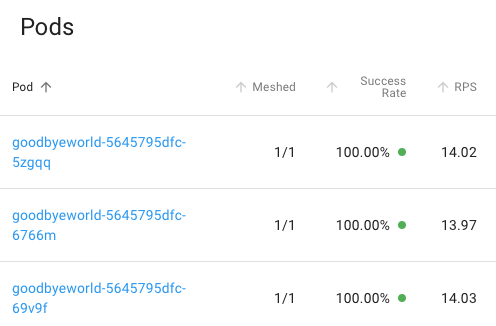
\includegraphics[width=\columnwidth]{img/results-load-balance}
	\caption{The \textsc{goodbye-world-service} deployment shows all three replicas balancing the request-load.}
	\label{fig:results-load-balance}
\end{figure}

\subsubsection{Central Monitoring and Logging}
\label{sec:log-result}
As we can see \linkerd{} comes with a dashboard showing the current state of the service mesh (see images in \autoref{sec:canary-result} and \autoref{sec:load-result}).
To collect the so called "golden metrics" \linkerd{} brings \textsc{Prometheus} which is out-of-box connected to each pod.
With this we can see \textit{who} is talking \textit{how much} to \textit{whom}.
Next to the \linkerd{} dashboard there is a \textsc{Grafana} component for each deployment \linkerd{} provides automatically.
Different from the dashboard of \linkerd{} \textsc{Grafana} shows temporal progression of the metrics.

To receive the logs of a service you may use the \kubernetes{} command \lstinline|kubectl logs <pod> <service>|
	\footnote{
		There was an own implementation for logs in \linkerd{} (\lstinline|linkerd logs|). 
		It was removed somewhere about version 2.4 since it overlapped with \lstinline|kubectl logs|.
		Read more in this GitHub discussion:\\
		\url{https://github.com/linkerd/linkerd2/discussions/5790}
	}.

\subsection{Pitfalls}
This section is for everybody wanting to reproduce showcases above.
Here we stated most important hints for which we would have been grateful if we had had them at the beginning:
\begin{itemize}
	\item First tip: Bring some time.\\
	To use \linkerd{} you have to acquire knowledge about \kubernetes{} and the Unix-Shell.
	There os no way to use \linkerd{} without \kubernetes{}.
	In many commands you rather have to call \lstinline|kubectl| than \lstinline|linkerd|.


	\item as you can see, we weren't able to apply access policies
\end{itemize}
\begin{itemize}
	\item \linkerd{} says, it'll need only 2GB of RAM 
	\begin{itemize}
		\item that was not enough. K8s was crashing
		\item With 4 GB it works
	\end{itemize}

	\item Minikube
	\begin{itemize}
		\item use command to build docker images into minikube-environment to be available in K8s.
		Remember to run this command in every shell you want to build \textsc{Docker}-images for \textsc{Minikube}:
		\lstinline|eval $(minikube -p minikube docker-env)|
		WHAT TOES IT DO? TBD
	\end{itemize}

	\item use bash-completion
	\kubernetes{} deploys pods with an unique name by appending an alphanumeric identifier to the service-name, as you can see in \autoref{fig:results-load-balance}.
	For making it easier to type these unique names into the CLI you can use \textsc{Bash-completion}
	
	\item Use ssh-port-forwarding to communicate with dashboard on VPS	
\end{itemize}

For further details on the setup, configuration and usage, see the appendix.



\section{Conclusion}

The theoretical and practical discussion of service meshes gave us very good impressions of the advantages and disadvantages of using them.
On the one hand, it is really very easy to apply or remove policies in the microservice architecture dynamically via customization of YAML resources. Powerful features such as circuit breaking, canary deployment, and centralized management ease the burden on both developers and operators of microservices architectures.

The proof of concept we presented using \textsc{Linkerd} hinted at the strengths and weaknesses of service meshes. It would certainly be interesting to take another look at \textsc{Istio}, as it promises a wider range of functions despite its higher complexity.

However, although \textsc{Linkerd} describes itself as lightweight, one aspect clearly emerged during the implementation of the proof of concept: The benefits of service meshes only come into play once the overall system is fully deployed. The creation of \textsc{Kubernetes} services and the commissioning of \textsc{Linkerd} require a high level of expert knowledge and effort. Consequently, it is rather utopian to integrate service meshes into a microservice landscape within a short time. However, once the first breakthrough has been achieved, the further development of new or existing microservices is comparatively more productive. The claim that developers can focus more on implementing the business logic is in line with our experience from dealing with \textsc{Linkerd}.
\begin{thebibliography}{00}

\bibitem{microservices-general} P. Giessler, ``Dom\"anengetriebener Entwurf von ressourcenorientierten Microservices'', Karlsruher Institut für Technologie (KIT), 2018

\bibitem{spring-cloud} 
Spring Cloud \url{https://spring.io/projects/spring-cloud} (Last access: 2021/02/11, 11 am)

\bibitem{from-monolith} R. Chen, S. Li and Z. Li, "From Monolith to Microservices: A Dataflow-Driven Approach," 2017 24th Asia-Pacific Software Engineering Conference (APSEC), Nanjing, 2017, p. 473

\bibitem{sm1} W. Li, Y. Lemieux, J. Gao, Z. Zhao and Y. Han, "Service Mesh: Challenges, State of the Art, and Future Research Opportunities," 2019 IEEE International Conference on Service-Oriented System Engineering (SOSE), San Francisco East Bay, CA, USA, 2019, pp. 122-1225

\bibitem{sm2} Was ist ein Service Mesh? - \url{https://www.redhat.com/de/topics/microservices/what-is-a-service-mesh} (Last access: 2021/02/11, 12 am)

\bibitem{sm3} Indrasiri, Kasun., and Prabath. Siriwardena. ``Microservices for the Enterprise": Designing, Developing, and Deploying / by Kasun Indrasiri, Prabath Siriwardena. 1st ed. 2018., Apress, 2018

\bibitem{sm4}
K. Y. Ponomarev, ``Attribute-Based Access Control in Service Mesh," 2019 Dynamics of Systems, Mechanisms and Machines (Dynamics), Omsk, Russia, 2019, pp. 1-4

\bibitem{linkerd-github} linkerd/linkerd2 @ GitHub - \url{https://github.com/linkerd/linkerd2} (Last access: 2021/02/17, 11 am)

\bibitem{istio-github} istio/istio @ GitHub - \url{https://github.com/istio/istio} (Last access: 2021/02/17, 11 am)

\bibitem{istio-linkerd-compare-1} Kubernetes Service Mesh: A Comparison of Istio, Linkerd and Consul - \url{https://platform9.com/blog/kubernetes-service-mesh-a-comparison-of-istio-linkerd-and-consul/} (Last access: 2021/02/17, 11 am)

\bibitem{istio-linkerd-compare-2} Service Mesh: Einführung \& Vergleich von Istio und Linkerd - \url{https://www.predic8.de/service-mesh-microservices.htm}  (Last access: 2021/02/17, 11 am)

\bibitem{linkerd-circuit-breaker} Circuit breaker support? - \url{https://github.com/linkerd/linkerd2/issues/2846} (Last access: 2021/02/17, 2 pm)

\bibitem{fowler} Microservices - \url{https://martinfowler.com/articles/microservices.html}

\bibitem{k8s} Konzepte | Kubernetes - \url{https://kubernetes.io/de/docs/concepts/}

\end{thebibliography}

\end{document}
